
\begin{frame}
	\frametitle{Estrés hídrico}
	
	\textbf{Nacionalmente:}
			
	\begin{itemize}
		\item En 2021 60 presas a menos del \qty{25}{\percent} \cite{national_aeronautics_and_space_administration_sequigeneralizada_2021} 
		\item Según el \acrshort{wri}, en 2021 México ocupaba el puesto 24 de 164 en mayor estrés hídrico
		\item Para 2040 estaremos en la categoría de \textit{extremely high-stress} \cite{maddocks_ranking_2015}
	\end{itemize}

		\begin{columns}
		\begin{column}{0.5\textwidth}
			\centering
			\begin{figure}
				\centering
				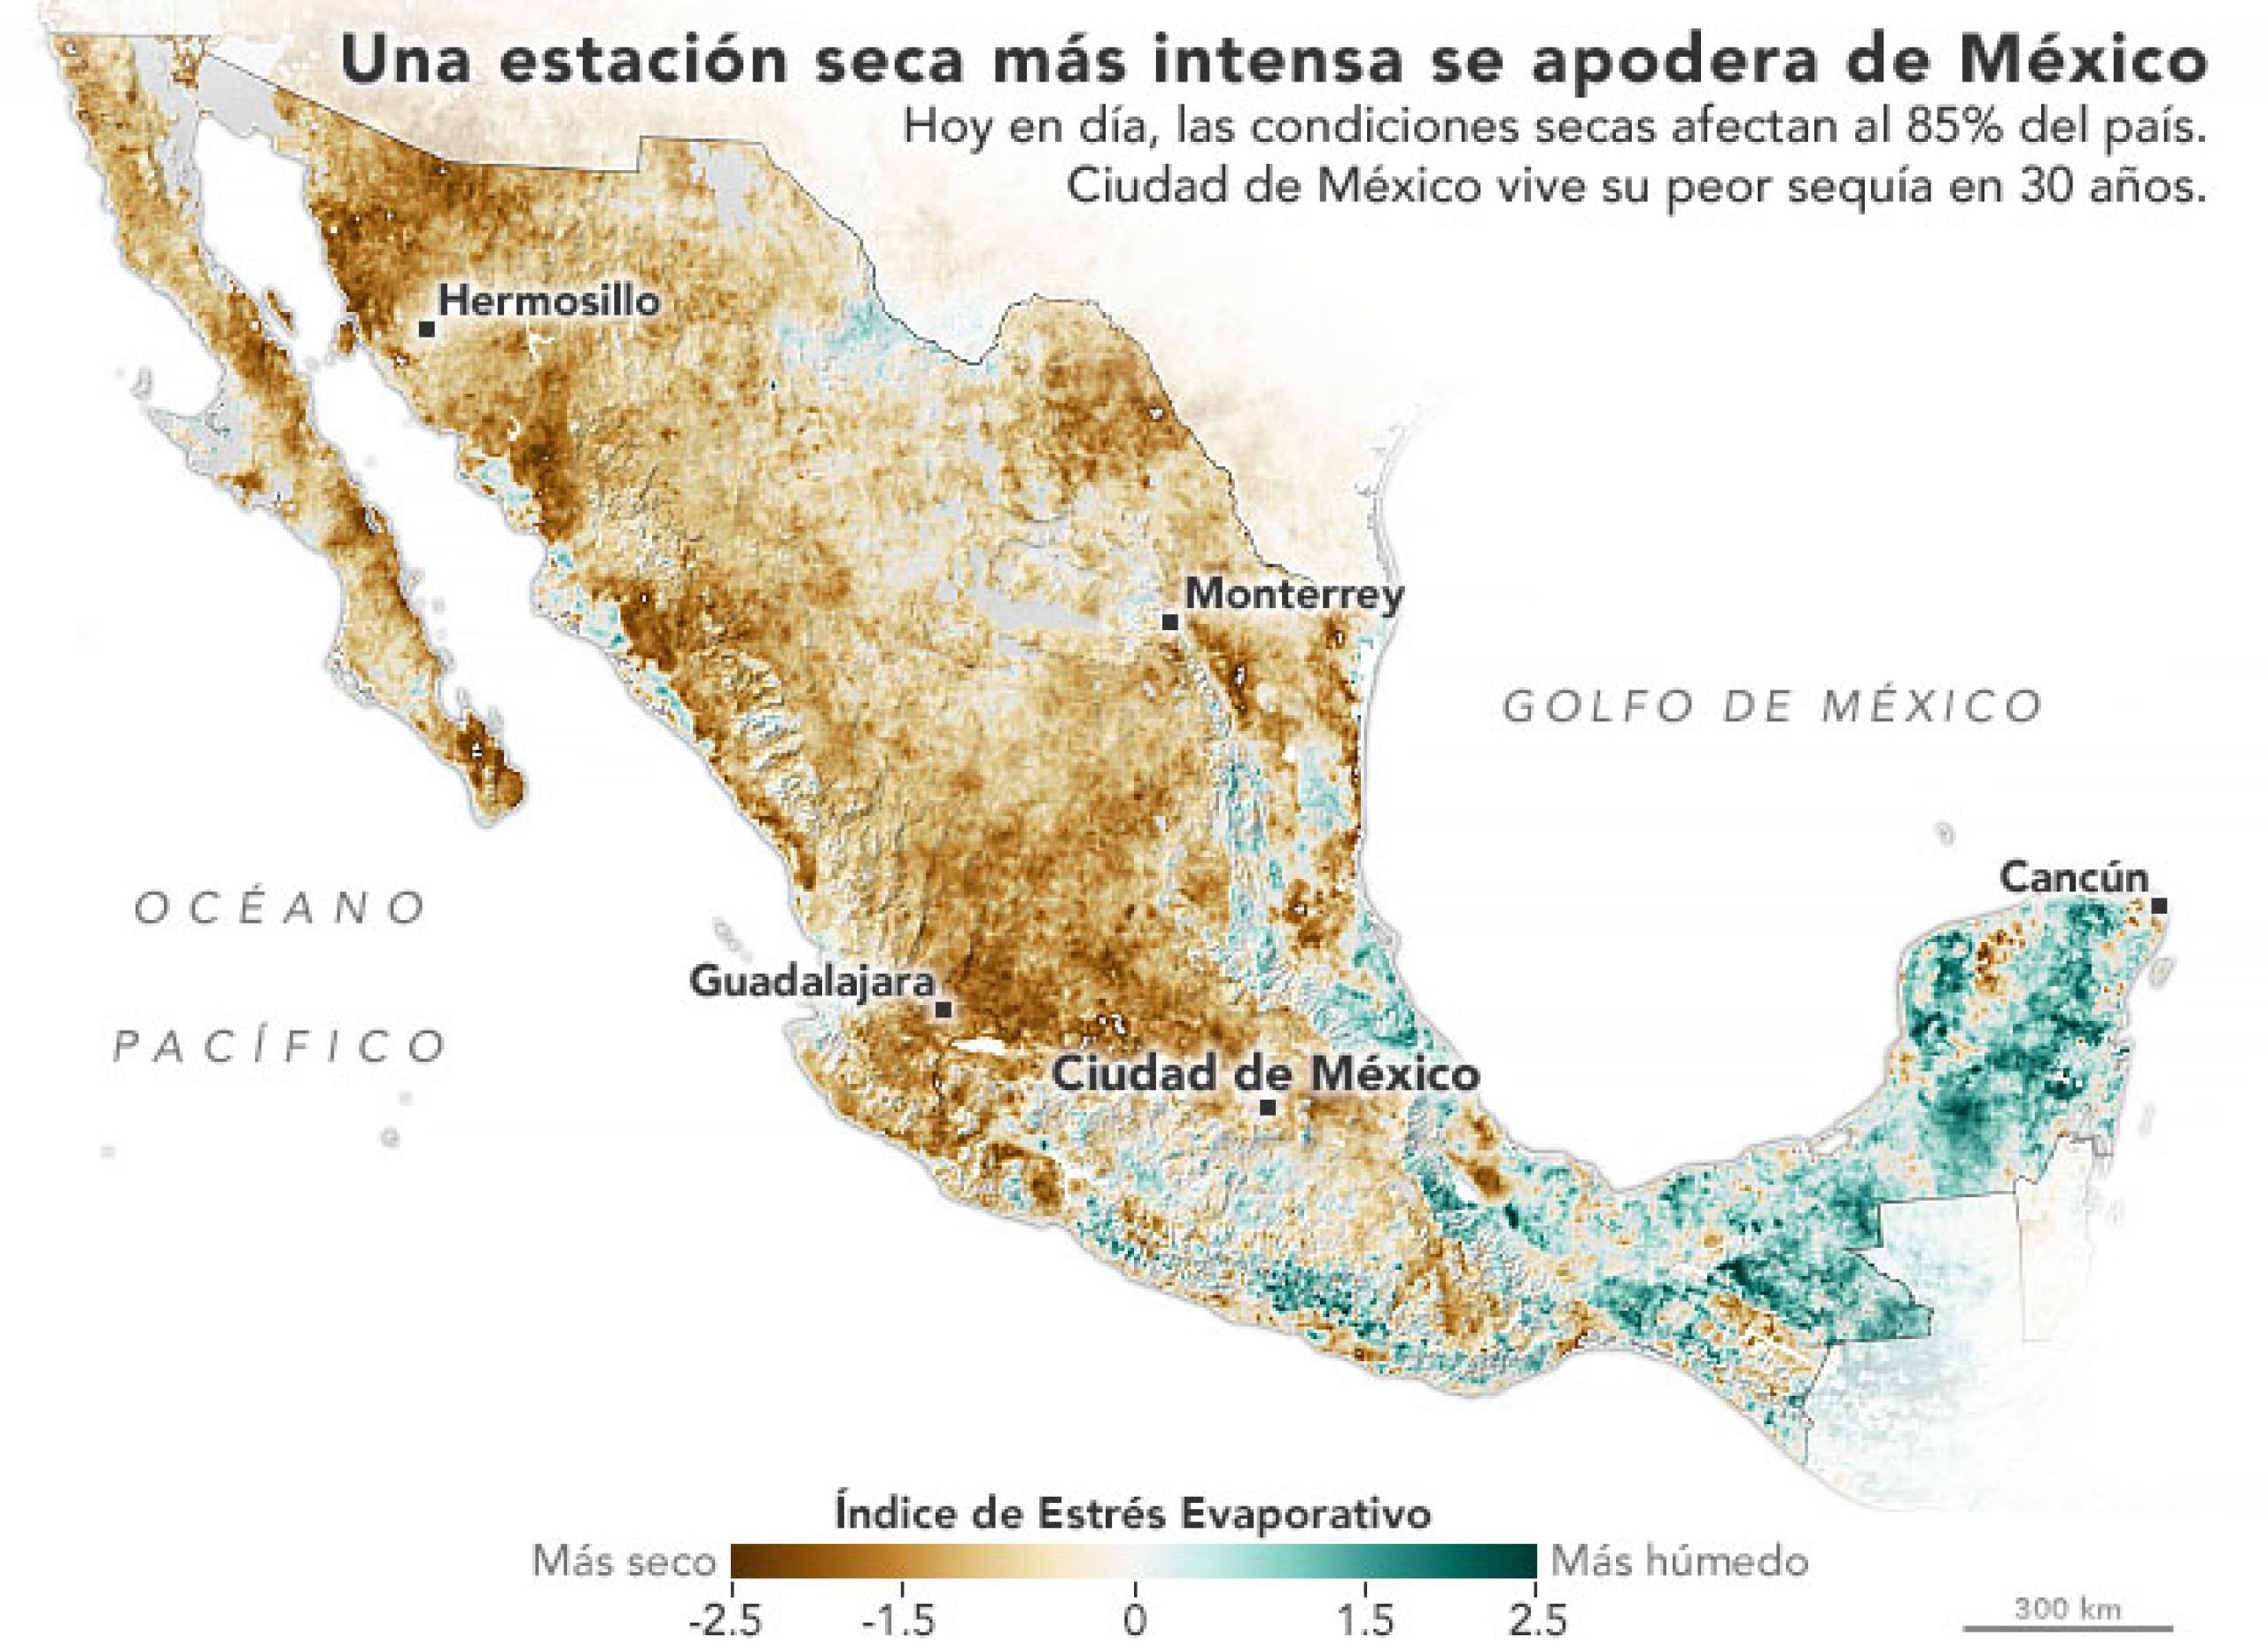
\includegraphics[
					height=35mm,
					width=\linewidth,
					keepaspectratio
				]{indice-estres-evaporativo.jpg}
				\caption{Índice de estrés evaporativo en México}
			\end{figure}
		\end{column}
		\begin{column}{0.5\textwidth}
			\centering
			\begin{figure}
				\centering
				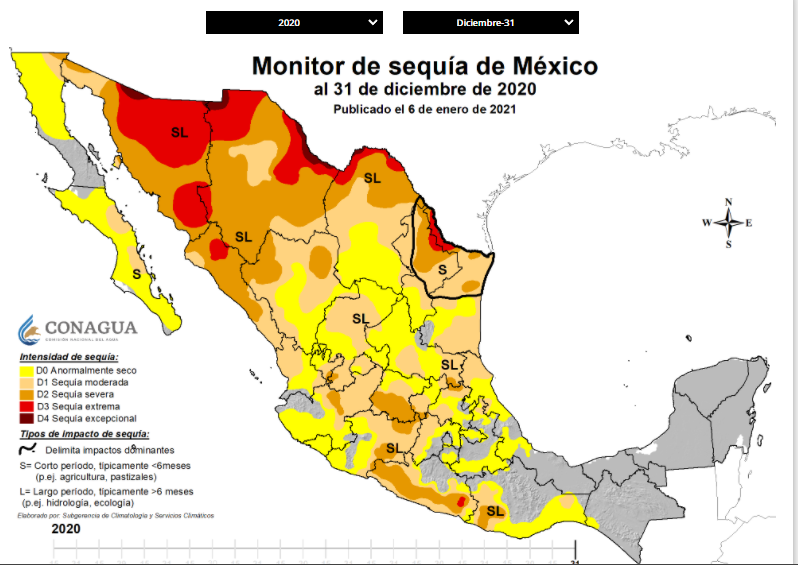
\includegraphics[
					height=35mm,
					width=\linewidth,
					keepaspectratio
				]{sequia2020.PNG}
				\caption{Monitor de sequía en México durante diciembre del 2020}
			\end{figure}
		\end{column}
	\end{columns}
\end{frame}